\chapter{Evaluación}
\label{cap:evaluacion}
Una vez terminado el desarrollo de AdaptaMaterialEscolar 2.0, llevamos a cabo una evaluación para evaluar si nuestro proyecto resultaba útil para los docentes que necesitaban realizar adaptaciones curriculares para sus estudiantes en cualquier etapa académica. Con el propósito de realizar una valoración detallada, nos enfocamos en evaluar varios aspectos de nuestro proyecto: el diseño de la interfaz, la usabilidad del sistema en su totalidad y de cada funcionalidad de manera independiente y detectar posibles mejoras que podrían implementarse en el futuro.

A continuación se explica el diseño de la evaluación (Sección \ref{sec:disenyoEvaluacion}), los resultados obtenidos  (Sección \ref{sec:resultadosEvaluacion}) y las conclusiones obtenidas (Sección \ref{sec:conclusionesEvaluacion}).

\section{Diseño}\label{sec:disenyoEvaluacion}
Con el fin de permitir a los usuarios finales evaluar nuestra aplicación, creamos un examen de prueba y una hoja de apuntes sobre las asignaturas de conocimiento del medio y matemáticas.
Para facilitar la evaluación y el análisis de los resultados de nuestra aplicación web, creamos una encuesta\footnote{\url{https://docs.google.com/forms/d/e/1FAIpQLSdg7mGUfGBW5LoGIWulEUq-vhloL5rlkU_aIZCUzpqiJp164A/viewform?usp=sf_link}} en Google Forms dirigida a los usuarios finales. Durante la evaluación, los usuarios experimentaban directamente con las diversas funcionalidades, tratando de replicar el examen y la hoja de apuntes proporcionados.

La evaluación se ha diseñado de la siguiente manera:
\begin{itemize}
    \item La evaluación comienza con varios párrafos agradeciendo la colaboración de los usuarios, explicando la herramienta que están a punto de probar y proporcionando un resumen de la estructura de la evaluación. Además, se solicitó a los usuarios que dieran su consentimiento para el tratamiento de los resultados obtenidos en la evaluación.
    \item A continuación, se realizarán unas preguntas de screening y demográficas para el posterior análisis de los datos.
          \begin{itemize}
              \item ¿Cuántos años tienes?
              \item ¿Eres docente?
          \end{itemize}
          ¿Eres estudiante de magisterio? 
          \begin{itemize}
              \item ¿Podrías decirnos en qué nivel del sistema educativo eres docente?
              \item ¿Has tenido que hacer alguna adaptación curricular no significativa?
              \item ¿Cuántas veces?
          \end{itemize}
    \item Después, el evaluador debía crear un examen con preguntas de todos los tipos posibles. En este apartado se les proporcionó a los usuarios un examen creado con AdaptaMaterialEscolar 2.0 para que tratasen de replicarlo. En el Apéndice \ref{ape:examenEvaluacion} se muestra el examen que se proporcionó a los usuarios para realizar la evaluación. Tras terminar de crear cada ejercicio, los usuarios debían responder a las siguientes preguntas de usabilidad:
          \begin{itemize}
              \item En general, estoy  satisfecho o satisfecha con la facilidad de completar esta tarea.
              \item En general estoy  satisfecho o satisfecha con la cantidad de tiempo que me ha llevado completar esta tarea.
              \item Estoy  satisfecho o satisfecha con la respuesta de la aplicación al realizar las acciones, sé lo que pasa en todo momento.
          \end{itemize}

          Tras finalizar el examen los usuarios debían exportar el documento de trabajo a PDF y subirlo al drive.

    \item A continuación, el evaluador debe crea unos apuntes que hagan uso de todas las funcionalidades de adaptación de textos. En este punto se les proporcionó a los usuarios una hoja de apuntes creada con AdaptaMaterialEscolar 2.0 para que tratasen de replicarla (en el Apéndice \ref{ape:examenEvaluacion} se muestra el examen que se proporcionó a los evaluadores). Después de cada adaptación, como en el caso anterior, los evaluadores debían responder al cuestionario ASQ. También se han realizado preguntas particulares para las funcionalidades de pictotraductor y generar resumen:
          \begin{itemize}
              \item PictoTraductor: 
              \begin{itemize}
                \item ¿La traducción resultante te parece correcta? 
                \item ¿Qué cuestiones crees que son mejorables en la traducción o que no son correctas?
              \end{itemize}
              \item Generación de resumen: 
              \begin{itemize}
                \item ¿El resumen resultante te parece correcto?
                \item ¿Qué cuestiones crees que son mejorables en el resumen o que no son correctas?
              \end{itemize}
          \end{itemize}
          Tras finalizar la hoja de apuntes los usuarios debían exportar el documento de trabajo a PDF y subirlo al drive.
    \item Una vez completadas las tareas de examen y de apuntes, se presentará un cuestionario con el objetivo de evaluar la facilidad de uso de la aplicación. En concreto, se utilizará el cuestionario Escala de Usabilidad de un Sistema\footnote{\url{https://uxpanol.com/teoria/sistema-de-escalas-de-usabilidad-que-es-y-para-que-sirve/}}, (SUS, por sus siglas en inglés). El cuestionario consta de las siguientes preguntas:
          \begin{itemize}
              \item Creo que usaría esta aplicación frecuentemente.
              \item Encontré la aplicación innecesariamente compleja.
              \item Creo que la aplicación es fácil de usar.
              \item Creo que necesitaría la ayuda de una persona con conocimientos técnicos para usar la aplicación.
              \item Las funciones de la aplicación están bien integradas.
              \item Creo que la aplicación es muy confusa.
              \item Creo que la mayoría de la gente aprendería a usar la aplicación muy rápidamente.
              \item Encuentro la aplicación muy complicada de utilizar.
              \item Me siento confiado o confiada al utilizar la aplicación.
              \item Necesito aprender muchas cosas antes de poder utilizar la aplicación.
          \end{itemize}
          Cada pregunta debe ser puntuada con una escala Likert de 5 puntos, donde 1 significa ``Muy en desacuerdo'' y 5 significa ``Muy de acuerdo''. Para calcular la puntuación final del SUS se debe utilizar la siguiente fórmula:
          \[[(SumaPreguntasImpares - 5) + (25 - SumaPreguntasPares)]\times2.5\]
          Esta fórmula, generará un valor en un rango de 0 a 100. Una puntuación de 0 indica una usabilidad extremadamente deficiente, lo que implica que el sistema evaluado es prácticamente inutilizable y presenta numerosos problemas o deficiencias. Por otro lado, una puntuación de 100 señala una usabilidad excepcionalmente alta, lo que implica que el sistema es altamente intuitivo, fácil de aprender y de utilizar.
    \item Finalmente, se llevaron a cabo varias preguntas generales de respuesta abierta con el objetivo de conocer mejor la opinión de los evaluadores sobre la aplicación y recibir sugerencias de mejora. Las preguntas son las siguientes:
          \begin{itemize}
              \item ¿Qué te ha parecido la aplicación?
              \item ¿Qué es lo que más te ha gustado?
              \item ¿Qué es lo que menos te ha gustado?
              \item ¿Echas de menos alguna funcionalidad?
              \item ¿Te sobra alguna funcionalidad?
              \item ¿Algo más que quieras añadir?
          \end{itemize}
\end{itemize}

\section{Resultados}\label{sec:resultadosEvaluacion}
La evaluación fue llevada a cabo por 5 docentes de Educación Infantil, Primaria, Secundaria o Bachillerato. A continuación se exponen los distintos resultados que se han obtenido en la evaluación.

En cuanto al apartado de la creación de un examen, los resultados obtenidos de cada tarea se muestran en las Tablas \ref{tab:resultadosVF}, \ref{tab:resultadosDefiniciones}, \ref{tab:resultadosDesarrollo}, \ref{tab:resultadoModificacion}, \ref{tab:resultadosCompletarHuecos}, \ref{tab:resultadosRelacionarConceptos}, \ref{tab:resultadosSopaLetras}, \ref{tab:resultadosMatematicas} y \ref{tab:resultadosEspacioDibujar}. En la Tabla \ref{tab:resultadosExamen} se muestran las medias de los resultados obtenidos en la creación del examen, que se han utilizado para generar la Figura \ref{fig:resultadosExamen}, en la cual se muestra una gráfica con la puntuación media de cada pregunta para cada ejercicio del examen.

\begin{table}[H]
    \resizebox{\textwidth}{!}{
        \begin{tabular}{c|ccc|l}
            \cline{2-4}
                                                     & \multicolumn{3}{c|}{\textbf{Ejercicio 1: Verdadero / Falso}}                                                                                                    &                                                                                                                                                                                                                                                                                                                                                                                \\ \cline{2-4}
                                                     & \multicolumn{1}{l|}{\textbf{\begin{tabular}[c]{@{}l@{}}1. En general, estoy satisfecho o satisfecha con \\ la facilidad de completar esta tarea.\end{tabular}}} & \multicolumn{1}{l|}{\textbf{\begin{tabular}[c]{@{}l@{}}2. En general estoy satisfecho o satisfecha con la cantidad \\ de tiempo que me ha llevado completar esta tarea.\end{tabular}}} & \textbf{\begin{tabular}[c]{@{}l@{}}3. Estoy satisfecho o satisfecha con la respuesta \\ de la aplicación al realizar las acciones, sé lo que \\ pasa en todo momento.\end{tabular}} & \\ \cline{1-4}
            \multicolumn{1}{|c|}{\textbf{Usuario 1}} & \multicolumn{1}{c|}{5}                                                                                                                                          & \multicolumn{1}{c|}{5}                                                                                                                                                                 & 5                                                                                                                                                                                   & \\ \cline{1-4}
            \multicolumn{1}{|c|}{\textbf{Usuario 2}} & \multicolumn{1}{c|}{5}                                                                                                                                          & \multicolumn{1}{c|}{4}                                                                                                                                                                 & 4                                                                                                                                                                                   & \\ \cline{1-4}
            \multicolumn{1}{|c|}{\textbf{Usuario 3}} & \multicolumn{1}{c|}{5}                                                                                                                                          & \multicolumn{1}{c|}{5}                                                                                                                                                                 & 5                                                                                                                                                                                   & \\ \cline{1-4}
            \multicolumn{1}{|c|}{\textbf{Usuario 4}} & \multicolumn{1}{c|}{5}                                                                                                                                          & \multicolumn{1}{c|}{5}                                                                                                                                                                 & 4                                                                                                                                                                                   & \\ \cline{1-4}
            \multicolumn{1}{|c|}{\textbf{Usuario 5}} & \multicolumn{1}{c|}{4}                                                                                                                                          & \multicolumn{1}{c|}{4}                                                                                                                                                                 & 4                                                                                                                                                                                   & \\ \cline{1-4}
            \multicolumn{1}{|c|}{\textbf{Media}}     & \multicolumn{1}{c|}{\textbf{4,8}}                                                                                                                               & \multicolumn{1}{c|}{\textbf{4,6}}                                                                                                                                                      & \textbf{4,4}                                                                                                                                                                        & \\ \cline{1-4}
        \end{tabular}
    }
    \caption{Resultados de ejercicio de verdadero / falso.}
    \label{tab:resultadosVF}
\end{table}

\begin{table}[H]
    \resizebox{\textwidth}{!}{
        \begin{tabular}{l|ccc|}
            \cline{2-4}
                                                     & \multicolumn{3}{c|}{\textbf{Ejercicio 2: Definiciones}}                                                                                                                                                                                                                                                                                                                                                                                                                                                                                                             \\ \cline{2-4}
                                                     & \multicolumn{1}{l|}{\textbf{\begin{tabular}[c]{@{}l@{}}1. En general, estoy satisfecho o satisfecha con \\ la facilidad de completar esta tarea.\end{tabular}}} & \multicolumn{1}{l|}{\textbf{\begin{tabular}[c]{@{}l@{}}2. En general estoy satisfecho o satisfecha con la cantidad \\ de tiempo que me ha llevado completar esta tarea.\end{tabular}}} & \multicolumn{1}{l|}{\textbf{\begin{tabular}[c]{@{}l@{}}3. Estoy satisfecho o satisfecha con la respuesta \\ de la aplicación al realizar las acciones, sé lo que \\ pasa en todo momento.\end{tabular}}} \\ \hline
            \multicolumn{1}{|l|}{\textbf{Usuario 1}} & \multicolumn{1}{c|}{5}                                                                                                                                          & \multicolumn{1}{c|}{5}                                                                                                                                                                 & 5                                                                                                                                                                                                        \\ \hline
            \multicolumn{1}{|l|}{\textbf{Usuario 2}} & \multicolumn{1}{c|}{5}                                                                                                                                          & \multicolumn{1}{c|}{4}                                                                                                                                                                 & 5                                                                                                                                                                                                        \\ \hline
            \multicolumn{1}{|l|}{\textbf{Usuario 3}} & \multicolumn{1}{c|}{3}                                                                                                                                          & \multicolumn{1}{c|}{4}                                                                                                                                                                 & 3                                                                                                                                                                                                        \\ \hline
            \multicolumn{1}{|l|}{\textbf{Usuario 4}} & \multicolumn{1}{c|}{5}                                                                                                                                          & \multicolumn{1}{c|}{5}                                                                                                                                                                 & 5                                                                                                                                                                                                        \\ \hline
            \multicolumn{1}{|l|}{\textbf{Usuario 5}} & \multicolumn{1}{c|}{5}                                                                                                                                          & \multicolumn{1}{c|}{5}                                                                                                                                                                 & 5                                                                                                                                                                                                        \\ \hline
            \multicolumn{1}{|c|}{\textbf{Media}}     & \multicolumn{1}{c|}{\textbf{4,6}}                                                                                                                               & \multicolumn{1}{c|}{\textbf{4,6}}                                                                                                                                                      & \textbf{4,6}                                                                                                                                                                                             \\ \hline
        \end{tabular}%
    }
    \caption{Resultados de ejercicio de definiciones.}
    \label{tab:resultadosDefiniciones}
\end{table}

\begin{table}[H]
    \resizebox{\textwidth}{!}{
        \begin{tabular}{c|ccc|l}
            \cline{2-4}
                                                     & \multicolumn{3}{c|}{\textbf{Ejercicio 3: Desarrollo}}                                                                                                           &                                                                                                                                                                                                                                                                                                                                                                                \\ \cline{2-4}
                                                     & \multicolumn{1}{l|}{\textbf{\begin{tabular}[c]{@{}l@{}}1. En general, estoy satisfecho o satisfecha con \\ la facilidad de completar esta tarea.\end{tabular}}} & \multicolumn{1}{l|}{\textbf{\begin{tabular}[c]{@{}l@{}}2. En general estoy satisfecho o satisfecha con la cantidad \\ de tiempo que me ha llevado completar esta tarea.\end{tabular}}} & \textbf{\begin{tabular}[c]{@{}l@{}}3. Estoy satisfecho o satisfecha con la respuesta \\ de la aplicación al realizar las acciones, sé lo que \\ pasa en todo momento.\end{tabular}} & \\ \cline{1-4}
            \multicolumn{1}{|c|}{\textbf{Usuario 1}} & \multicolumn{1}{c|}{5}                                                                                                                                          & \multicolumn{1}{c|}{5}                                                                                                                                                                 & 5                                                                                                                                                                                   & \\ \cline{1-4}
            \multicolumn{1}{|c|}{\textbf{Usuario 2}} & \multicolumn{1}{c|}{5}                                                                                                                                          & \multicolumn{1}{c|}{5}                                                                                                                                                                 & 5                                                                                                                                                                                   & \\ \cline{1-4}
            \multicolumn{1}{|c|}{\textbf{Usuario 3}} & \multicolumn{1}{c|}{5}                                                                                                                                          & \multicolumn{1}{c|}{5}                                                                                                                                                                 & 5                                                                                                                                                                                   & \\ \cline{1-4}
            \multicolumn{1}{|c|}{\textbf{Usuario 4}} & \multicolumn{1}{c|}{5}                                                                                                                                          & \multicolumn{1}{c|}{5}                                                                                                                                                                 & 5                                                                                                                                                                                   & \\ \cline{1-4}
            \multicolumn{1}{|c|}{\textbf{Usuario 5}} & \multicolumn{1}{c|}{5}                                                                                                                                          & \multicolumn{1}{c|}{5}                                                                                                                                                                 & 5                                                                                                                                                                                   & \\ \cline{1-4}
            \multicolumn{1}{|c|}{\textbf{Media}}     & \multicolumn{1}{c|}{\textbf{5}}                                                                                                                                 & \multicolumn{1}{c|}{\textbf{5}}                                                                                                                                                        & \textbf{5}                                                                                                                                                                          & \\ \cline{1-4}
        \end{tabular}
    }
    \caption{Resultados de ejercicio de desarrollo.}
    \label{tab:resultadosDesarrollo}
\end{table}

\begin{table}[H]
    \resizebox{\textwidth}{!}{
        \begin{tabular}{c|ccc|l}
            \cline{2-4}
                                                     & \multicolumn{3}{c|}{\textbf{Modificación del ejercicio de desarrollo}}                                                                                          &                                                                                                                                                                                                                                                                                                                                                                                                     \\ \cline{2-4}
                                                     & \multicolumn{1}{l|}{\textbf{\begin{tabular}[c]{@{}l@{}}1. En general, estoy satisfecho o satisfecha con \\ la facilidad de completar esta tarea.\end{tabular}}} & \multicolumn{1}{l|}{\textbf{\begin{tabular}[c]{@{}l@{}}2. En general estoy satisfecho o satisfecha con la cantidad \\ de tiempo que me ha llevado completar esta tarea.\end{tabular}}} & \multicolumn{1}{l|}{\textbf{\begin{tabular}[c]{@{}l@{}}3. Estoy satisfecho o satisfecha con la respuesta \\ de la aplicación al realizar las acciones, sé lo que \\ pasa en todo momento.\end{tabular}}} & \\ \cline{1-4}
            \multicolumn{1}{|c|}{\textbf{Usuario 1}} & \multicolumn{1}{c|}{5}                                                                                                                                          & \multicolumn{1}{c|}{5}                                                                                                                                                                 & 5                                                                                                                                                                                                        & \\ \cline{1-4}
            \multicolumn{1}{|c|}{\textbf{Usuario 2}} & \multicolumn{1}{c|}{5}                                                                                                                                          & \multicolumn{1}{c|}{5}                                                                                                                                                                 & 5                                                                                                                                                                                                        & \\ \cline{1-4}
            \multicolumn{1}{|c|}{\textbf{Usuario 3}} & \multicolumn{1}{c|}{5}                                                                                                                                          & \multicolumn{1}{c|}{5}                                                                                                                                                                 & 5                                                                                                                                                                                                        & \\ \cline{1-4}
            \multicolumn{1}{|c|}{\textbf{Usuario 4}} & \multicolumn{1}{c|}{5}                                                                                                                                          & \multicolumn{1}{c|}{5}                                                                                                                                                                 & 5                                                                                                                                                                                                        & \\ \cline{1-4}
            \multicolumn{1}{|c|}{\textbf{Usuario 5}} & \multicolumn{1}{c|}{5}                                                                                                                                          & \multicolumn{1}{c|}{5}                                                                                                                                                                 & 5                                                                                                                                                                                                        & \\ \cline{1-4}
            \multicolumn{1}{|c|}{\textbf{Media}}     & \multicolumn{1}{c|}{\textbf{5}}                                                                                                                                 & \multicolumn{1}{c|}{\textbf{5}}                                                                                                                                                        & \textbf{5}                                                                                                                                                                                               & \\ \cline{1-4}
        \end{tabular}
    }
    \caption{Resultados de modificación de ejercicio de desarrollo.}
    \label{tab:resultadoModificacion}
\end{table}

\begin{table}[H]
    \resizebox{\textwidth}{!}{
        \begin{tabular}{l|ccc|}
            \cline{2-4}
                                                     & \multicolumn{3}{c|}{\textbf{Ejercicio 4: Completar huecos}}                                                                                                                                                                                                                                                                                                                                                                                                                                                                                                         \\ \cline{2-4}
                                                     & \multicolumn{1}{l|}{\textbf{\begin{tabular}[c]{@{}l@{}}1. En general, estoy satisfecho o satisfecha con \\ la facilidad de completar esta tarea.\end{tabular}}} & \multicolumn{1}{l|}{\textbf{\begin{tabular}[c]{@{}l@{}}2. En general estoy satisfecho o satisfecha con la cantidad \\ de tiempo que me ha llevado completar esta tarea.\end{tabular}}} & \multicolumn{1}{l|}{\textbf{\begin{tabular}[c]{@{}l@{}}3. Estoy satisfecho o satisfecha con la respuesta \\ de la aplicación al realizar las acciones, sé lo que \\ pasa en todo momento.\end{tabular}}} \\ \hline
            \multicolumn{1}{|l|}{\textbf{Usuario 1}} & \multicolumn{1}{c|}{5}                                                                                                                                          & \multicolumn{1}{c|}{5}                                                                                                                                                                 & 5                                                                                                                                                                                                        \\ \hline
            \multicolumn{1}{|l|}{\textbf{Usuario 2}} & \multicolumn{1}{c|}{5}                                                                                                                                          & \multicolumn{1}{c|}{5}                                                                                                                                                                 & 5                                                                                                                                                                                                        \\ \hline
            \multicolumn{1}{|l|}{\textbf{Usuario 3}} & \multicolumn{1}{c|}{5}                                                                                                                                          & \multicolumn{1}{c|}{5}                                                                                                                                                                 & 5                                                                                                                                                                                                        \\ \hline
            \multicolumn{1}{|l|}{\textbf{Usuario 4}} & \multicolumn{1}{c|}{5}                                                                                                                                          & \multicolumn{1}{c|}{5}                                                                                                                                                                 & 5                                                                                                                                                                                                        \\ \hline
            \multicolumn{1}{|l|}{\textbf{Usuario 5}} & \multicolumn{1}{c|}{5}                                                                                                                                          & \multicolumn{1}{c|}{5}                                                                                                                                                                 & 5                                                                                                                                                                                                        \\ \hline
            \multicolumn{1}{|c|}{\textbf{Media}}     & \multicolumn{1}{c|}{\textbf{5}}                                                                                                                                 & \multicolumn{1}{c|}{\textbf{5}}                                                                                                                                                        & \textbf{5}                                                                                                                                                                                               \\ \hline
        \end{tabular}
    }
    \caption{Resultados de ejercicio de completar huecos.}
    \label{tab:resultadosCompletarHuecos}
\end{table}

\begin{table}[H]
    \resizebox{\textwidth}{!}{
        \begin{tabular}{c|ccc|l}
            \cline{2-4}
                                                     & \multicolumn{3}{c|}{\textbf{Ejercicio 5: Relacionar conceptos}}                                                                                                 &                                                                                                                                                                                                                                                                                                                                                                                                     \\ \cline{2-4}
                                                     & \multicolumn{1}{l|}{\textbf{\begin{tabular}[c]{@{}l@{}}1. En general, estoy satisfecho o satisfecha con \\ la facilidad de completar esta tarea.\end{tabular}}} & \multicolumn{1}{l|}{\textbf{\begin{tabular}[c]{@{}l@{}}2. En general estoy satisfecho o satisfecha con la cantidad \\ de tiempo que me ha llevado completar esta tarea.\end{tabular}}} & \multicolumn{1}{l|}{\textbf{\begin{tabular}[c]{@{}l@{}}3. Estoy satisfecho o satisfecha con la respuesta \\ de la aplicación al realizar las acciones, sé lo que \\ pasa en todo momento.\end{tabular}}} & \\ \cline{1-4}
            \multicolumn{1}{|c|}{\textbf{Usuario 1}} & \multicolumn{1}{c|}{5}                                                                                                                                          & \multicolumn{1}{c|}{5}                                                                                                                                                                 & 5                                                                                                                                                                                                        & \\ \cline{1-4}
            \multicolumn{1}{|c|}{\textbf{Usuario 2}} & \multicolumn{1}{c|}{5}                                                                                                                                          & \multicolumn{1}{c|}{5}                                                                                                                                                                 & 5                                                                                                                                                                                                        & \\ \cline{1-4}
            \multicolumn{1}{|c|}{\textbf{Usuario 3}} & \multicolumn{1}{c|}{4}                                                                                                                                          & \multicolumn{1}{c|}{5}                                                                                                                                                                 & 4                                                                                                                                                                                                        & \\ \cline{1-4}
            \multicolumn{1}{|c|}{\textbf{Usuario 4}} & \multicolumn{1}{c|}{5}                                                                                                                                          & \multicolumn{1}{c|}{5}                                                                                                                                                                 & 5                                                                                                                                                                                                        & \\ \cline{1-4}
            \multicolumn{1}{|c|}{\textbf{Usuario 5}} & \multicolumn{1}{c|}{4}                                                                                                                                          & \multicolumn{1}{c|}{4}                                                                                                                                                                 & 4                                                                                                                                                                                                        & \\ \cline{1-4}
            \multicolumn{1}{|c|}{\textbf{Media}}     & \multicolumn{1}{c|}{\textbf{4,6}}                                                                                                                               & \multicolumn{1}{c|}{\textbf{4,8}}                                                                                                                                                      & \textbf{4,6}                                                                                                                                                                                             & \\ \cline{1-4}
        \end{tabular}
    }
    \caption{Resultados de ejercicio de relacionar conceptos.}
    \label{tab:resultadosRelacionarConceptos}
\end{table}

\begin{table}[H]
    \resizebox{\textwidth}{!}{%
        \begin{tabular}{l|ccc|}
            \cline{2-4}
                                                     & \multicolumn{3}{c|}{\textbf{Ejercicio 6: Sopa de letras}}                                                                                                                                                                                                                                                                                                                                                                                                                                                                                                           \\ \cline{2-4}
                                                     & \multicolumn{1}{l|}{\textbf{\begin{tabular}[c]{@{}l@{}}1. En general, estoy satisfecho o satisfecha con \\ la facilidad de completar esta tarea.\end{tabular}}} & \multicolumn{1}{l|}{\textbf{\begin{tabular}[c]{@{}l@{}}2. En general estoy satisfecho o satisfecha con la cantidad \\ de tiempo que me ha llevado completar esta tarea.\end{tabular}}} & \multicolumn{1}{l|}{\textbf{\begin{tabular}[c]{@{}l@{}}3. Estoy satisfecho o satisfecha con la respuesta \\ de la aplicación al realizar las acciones, sé lo que \\ pasa en todo momento.\end{tabular}}} \\ \hline
            \multicolumn{1}{|l|}{\textbf{Usuario 1}} & \multicolumn{1}{c|}{5}                                                                                                                                          & \multicolumn{1}{c|}{5}                                                                                                                                                                 & 5                                                                                                                                                                                                        \\ \hline
            \multicolumn{1}{|l|}{\textbf{Usuario 2}} & \multicolumn{1}{c|}{5}                                                                                                                                          & \multicolumn{1}{c|}{5}                                                                                                                                                                 & 5                                                                                                                                                                                                        \\ \hline
            \multicolumn{1}{|l|}{\textbf{Usuario 3}} & \multicolumn{1}{c|}{5}                                                                                                                                          & \multicolumn{1}{c|}{5}                                                                                                                                                                 & 5                                                                                                                                                                                                        \\ \hline
            \multicolumn{1}{|l|}{\textbf{Usuario 4}} & \multicolumn{1}{c|}{5}                                                                                                                                          & \multicolumn{1}{c|}{5}                                                                                                                                                                 & 5                                                                                                                                                                                                        \\ \hline
            \multicolumn{1}{|l|}{\textbf{Usuario 5}} & \multicolumn{1}{c|}{5}                                                                                                                                          & \multicolumn{1}{c|}{5}                                                                                                                                                                 & 5                                                                                                                                                                                                        \\ \hline
            \multicolumn{1}{|c|}{\textbf{Media}}     & \multicolumn{1}{c|}{\textbf{5}}                                                                                                                                 & \multicolumn{1}{c|}{\textbf{5}}                                                                                                                                                        & \textbf{5}                                                                                                                                                                                               \\ \hline
        \end{tabular}
    }
    \caption{Resultados de ejercicio de sopa de letras.}
    \label{tab:resultadosSopaLetras}
\end{table}

\begin{table}[H]
    \resizebox{\textwidth}{!}{
        \begin{tabular}{c|ccc|l}
            \cline{2-4}
                                                     & \multicolumn{3}{c|}{\textbf{Ejercicio 7: Matemáticas}}                                                                                                          &                                                                                                                                                                                                                                                                                                                                                                                                     \\ \cline{2-4}
                                                     & \multicolumn{1}{l|}{\textbf{\begin{tabular}[c]{@{}l@{}}1. En general, estoy satisfecho o satisfecha con \\ la facilidad de completar esta tarea.\end{tabular}}} & \multicolumn{1}{l|}{\textbf{\begin{tabular}[c]{@{}l@{}}2. En general estoy satisfecho o satisfecha con la cantidad \\ de tiempo que me ha llevado completar esta tarea.\end{tabular}}} & \multicolumn{1}{l|}{\textbf{\begin{tabular}[c]{@{}l@{}}3. Estoy satisfecho o satisfecha con la respuesta \\ de la aplicación al realizar las acciones, sé lo que \\ pasa en todo momento.\end{tabular}}} & \\ \cline{1-4}
            \multicolumn{1}{|c|}{\textbf{Usuario 1}} & \multicolumn{1}{c|}{4}                                                                                                                                          & \multicolumn{1}{c|}{5}                                                                                                                                                                 & 5                                                                                                                                                                                                        & \\ \cline{1-4}
            \multicolumn{1}{|c|}{\textbf{Usuario 2}} & \multicolumn{1}{c|}{4}                                                                                                                                          & \multicolumn{1}{c|}{5}                                                                                                                                                                 & 5                                                                                                                                                                                                        & \\ \cline{1-4}
            \multicolumn{1}{|c|}{\textbf{Usuario 3}} & \multicolumn{1}{c|}{4}                                                                                                                                          & \multicolumn{1}{c|}{5}                                                                                                                                                                 & 3                                                                                                                                                                                                        & \\ \cline{1-4}
            \multicolumn{1}{|c|}{\textbf{Usuario 4}} & \multicolumn{1}{c|}{4}                                                                                                                                          & \multicolumn{1}{c|}{4}                                                                                                                                                                 & 3                                                                                                                                                                                                        & \\ \cline{1-4}
            \multicolumn{1}{|c|}{\textbf{Usuario 5}} & \multicolumn{1}{c|}{1}                                                                                                                                          & \multicolumn{1}{c|}{1}                                                                                                                                                                 & 1                                                                                                                                                                                                        & \\ \cline{1-4}
            \multicolumn{1}{|c|}{\textbf{Media}}     & \multicolumn{1}{c|}{\textbf{3,4}}                                                                                                                               & \multicolumn{1}{c|}{\textbf{4}}                                                                                                                                                        & \textbf{3,4}                                                                                                                                                                                             & \\ \cline{1-4}
        \end{tabular}%
    }
    \caption{Resultados de ejercicio de matemáticas.}
    \label{tab:resultadosMatematicas}
\end{table}

\begin{table}[H]
    \resizebox{\textwidth}{!}{
        \begin{tabular}{l|ccc|}
            \cline{2-4}
                                                     & \multicolumn{3}{c|}{\textbf{Ejercicio 8: Espacio para dibujar}}                                                                                                                                                                                                                                                                                                                                                                                                                                                                                                     \\ \cline{2-4}
                                                     & \multicolumn{1}{l|}{\textbf{\begin{tabular}[c]{@{}l@{}}1. En general, estoy satisfecho o satisfecha con \\ la facilidad de completar esta tarea.\end{tabular}}} & \multicolumn{1}{l|}{\textbf{\begin{tabular}[c]{@{}l@{}}2. En general estoy satisfecho o satisfecha con la cantidad \\ de tiempo que me ha llevado completar esta tarea.\end{tabular}}} & \multicolumn{1}{l|}{\textbf{\begin{tabular}[c]{@{}l@{}}3. Estoy satisfecho o satisfecha con la respuesta \\ de la aplicación al realizar las acciones, sé lo que \\ pasa en todo momento.\end{tabular}}} \\ \hline
            \multicolumn{1}{|l|}{\textbf{Usuario 1}} & \multicolumn{1}{c|}{5}                                                                                                                                          & \multicolumn{1}{c|}{5}                                                                                                                                                                 & 5                                                                                                                                                                                                        \\ \hline
            \multicolumn{1}{|l|}{\textbf{Usuario 2}} & \multicolumn{1}{c|}{5}                                                                                                                                          & \multicolumn{1}{c|}{5}                                                                                                                                                                 & 5                                                                                                                                                                                                        \\ \hline
            \multicolumn{1}{|l|}{\textbf{Usuario 3}} & \multicolumn{1}{c|}{5}                                                                                                                                          & \multicolumn{1}{c|}{5}                                                                                                                                                                 & 5                                                                                                                                                                                                        \\ \hline
            \multicolumn{1}{|l|}{\textbf{Usuario 4}} & \multicolumn{1}{c|}{5}                                                                                                                                          & \multicolumn{1}{c|}{5}                                                                                                                                                                 & 5                                                                                                                                                                                                        \\ \hline
            \multicolumn{1}{|l|}{\textbf{Usuario 5}} & \multicolumn{1}{c|}{5}                                                                                                                                          & \multicolumn{1}{c|}{5}                                                                                                                                                                 & 5                                                                                                                                                                                                        \\ \hline
            \multicolumn{1}{|c|}{\textbf{Media}}     & \multicolumn{1}{c|}{\textbf{5}}                                                                                                                                 & \multicolumn{1}{c|}{\textbf{5}}                                                                                                                                                        & \textbf{5}                                                                                                                                                                                               \\ \hline
        \end{tabular}
    }
    \caption{Resultados de ejercicio con espacio para dibujar.}
    \label{tab:resultadosEspacioDibujar}
\end{table}

\begin{table}[H]
    \resizebox{\textwidth}{!}{
        \begin{tabular}{l|c|c|c|}
            \cline{2-4}
                                                                                                                               & \textbf{\begin{tabular}[c]{@{}l@{}}1. En general, estoy satisfecho o satisfecha \\ con la facilidad de completar esta tarea.\end{tabular}} & \textbf{\begin{tabular}[c]{@{}l@{}}2.   En general estoy satisfecho o satisfecha \\ con la cantidad de tiempo que me ha   llevado \\ completar esta tarea.\end{tabular}} & \textbf{\begin{tabular}[c]{@{}l@{}}3.   Estoy satisfecho o satisfecha con \\ la respuesta de la aplicación al realizar \\ las acciones, sé lo que pasa en todo \\ momento.\end{tabular}} \\ \hline
            \multicolumn{1}{|l|}{\textbf{\begin{tabular}[c]{@{}l@{}}Ejercicio de \\ Verdadero/Falso\end{tabular}}}             & 4,8                                                                                                                                        & 4,6                                                                                                                                                                      & 4,4                                                                                                                                                                                      \\ \hline
            \multicolumn{1}{|l|}{\textbf{Ejercicio de definiciones}}                                                           & 4,6                                                                                                                                        & 4,6                                                                                                                                                                      & 4,6                                                                                                                                                                                      \\ \hline
            \multicolumn{1}{|l|}{\textbf{Ejercicio de desarrollo}}                                                             & 5                                                                                                                                          & 5                                                                                                                                                                        & 5                                                                                                                                                                                        \\ \hline
            \multicolumn{1}{|l|}{\textbf{\begin{tabular}[c]{@{}l@{}}Modificación del \\ ejercicio de desarrollo\end{tabular}}} & 5                                                                                                                                          & 5                                                                                                                                                                        & 5                                                                                                                                                                                        \\ \hline
            \multicolumn{1}{|l|}{\textbf{\begin{tabular}[c]{@{}l@{}}Ejercicio de \\ completar huecos\end{tabular}}}            & 5                                                                                                                                          & 5                                                                                                                                                                        & 5                                                                                                                                                                                        \\ \hline
            \multicolumn{1}{|l|}{\textbf{\begin{tabular}[c]{@{}l@{}}Ejercicio de relacionar \\ conceptos\end{tabular}}}        & 4,6                                                                                                                                        & 4,8                                                                                                                                                                      & 4,6                                                                                                                                                                                      \\ \hline
            \multicolumn{1}{|l|}{\textbf{Ejercicio de sopa de letras}}                                                         & 5                                                                                                                                          & 5                                                                                                                                                                        & 5                                                                                                                                                                                        \\ \hline
            \multicolumn{1}{|l|}{\textbf{Ejercicio de matemáticas}}                                                            & 3,4                                                                                                                                        & 4                                                                                                                                                                        & 3,4                                                                                                                                                                                      \\ \hline
            \multicolumn{1}{|l|}{\textbf{\begin{tabular}[c]{@{}l@{}}Ejercicio de espacios \\ para dibujar\end{tabular}}}       & 5                                                                                                                                          & 5                                                                                                                                                                        & 5                                                                                                                                                                                        \\ \hline
        \end{tabular}
    }
    \caption{Resultados del apartado de creación de examen.}
    \label{tab:resultadosExamen}
\end{table}

\begin{figure}[ht!]
    \centering
    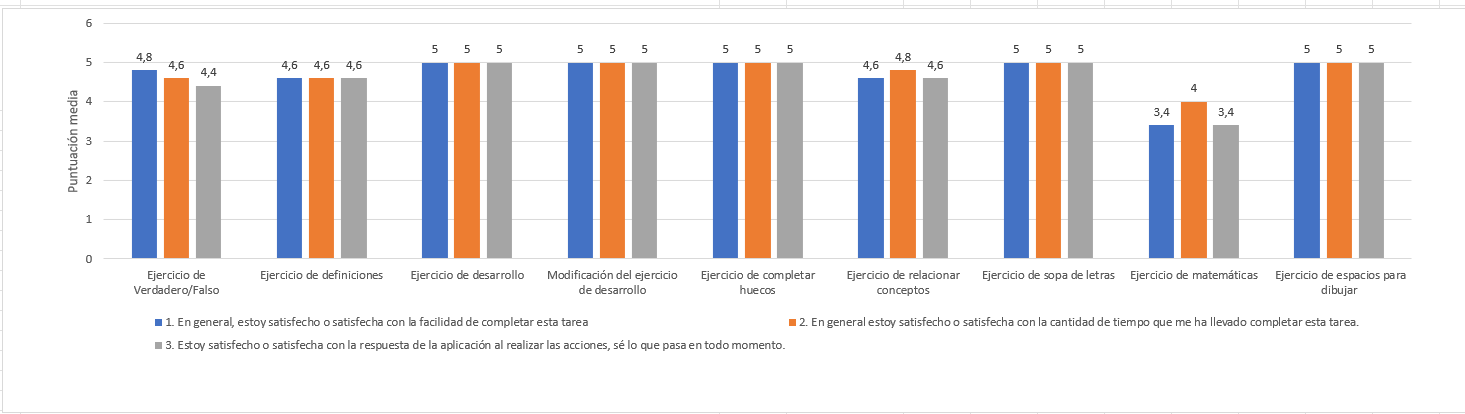
\includegraphics[width=0.8\textwidth]{Evaluacion/GraficaResultadosExamen.png}
    \caption{Resultados de creación del examen.}
    \label{fig:resultadosExamen}
\end{figure}

En cuanto al apartado de la creación de una hoja de apuntes, los resultados obtenidos de cada tarea se muestran en las Tablas \ref{tab:resultadosResumen}, \ref{tab:resultadosLeyendaColores}, \ref{tab:resultadosPictotraductor}, \ref{tab:resultdadosBorrar} y \ref{tab:resultadosBuscarPictogramas}.

\begin{table}[H]
    \resizebox{\textwidth}{!}{
        \begin{tabular}{c|ccccc|}
            \cline{2-6}
            \multicolumn{1}{l|}{}                    & \multicolumn{5}{c|}{\textbf{Actividad 1: Resumen}}                                                                                                                                                                                                                                                                                                                                                                                                                                                                                                                                                                                                                                                                                                                                                                                                                                                              \\ \cline{2-6}
            \multicolumn{1}{l|}{}                    & \multicolumn{1}{c|}{\textbf{\begin{tabular}[c]{@{}c@{}}¿El resumen resultante \\ te parece correcto?\end{tabular}}} & \multicolumn{1}{c|}{\textbf{\begin{tabular}[c]{@{}c@{}}¿Qué cuestiones crees \\ que son mejorables en \\ el resumen o que no \\ son correctas?\end{tabular}}}               & \multicolumn{1}{c|}{\textbf{\begin{tabular}[c]{@{}c@{}}1.   En general, estoy \\ satisfecho o \\ satisfecha con la facilidad\\  de completar \\ esta   tarea.\end{tabular}}} & \multicolumn{1}{c|}{\textbf{\begin{tabular}[c]{@{}c@{}}2.   En general estoy \\ satisfecho o \\ satisfecha con la cantidad \\ de tiempo \\ que me ha  llevado \\ completar esta tarea.\end{tabular}}} & \multicolumn{1}{l|}{\textbf{\begin{tabular}[c]{@{}l@{}}3.   Estoy satisfecho o \\ satisfecha con la respuesta \\ de la aplicación al \\ realizar  las acciones, \\ sé lo que pasa en todo \\ momento.\end{tabular}}} \\ \hline
            \multicolumn{1}{|l|}{\textbf{Usuario 1}} & \multicolumn{1}{c|}{No}                                                                                             & \multicolumn{1}{c|}{\begin{tabular}[c]{@{}c@{}}Está   muy bien. Lo ha resumido \\ mejor de lo que pensaba\end{tabular}}                                                     & \multicolumn{1}{c|}{5}                                                                                                                                                       & \multicolumn{1}{c|}{5}                                                                                                                                                                                & 5                                                                                                                                                                                                                    \\ \hline
            \multicolumn{1}{|c|}{\textbf{Usuario 2}} & \multicolumn{1}{c|}{Sí}                                                                                             & \multicolumn{1}{c|}{\begin{tabular}[c]{@{}c@{}}Es   mejorable la redacción \\ en cuanto a signos de \\ puntuación y conectores para \\ dar cohesión al texto.\end{tabular}} & \multicolumn{1}{c|}{5}                                                                                                                                                       & \multicolumn{1}{c|}{5}                                                                                                                                                                                & 5                                                                                                                                                                                                                    \\ \hline
            \multicolumn{1}{|c|}{\textbf{Usuario 3}} & \multicolumn{1}{c|}{Sí}                                                                                             & \multicolumn{1}{c|}{\begin{tabular}[c]{@{}c@{}}No   he visto dónde especificar \\ que quería 100 palabras.\end{tabular}}                                                    & \multicolumn{1}{c|}{3}                                                                                                                                                       & \multicolumn{1}{c|}{3}                                                                                                                                                                                & 3                                                                                                                                                                                                                    \\ \hline
            \multicolumn{1}{|c|}{\textbf{Usuario 4}} & \multicolumn{1}{c|}{Sí}                                                                                             & \multicolumn{1}{c|}{\begin{tabular}[c]{@{}c@{}}Se   podrían seleccionar \\ palabras que deseemos \\ que salgan obligatoriamente en \\ el resumen.\end{tabular}}             & \multicolumn{1}{c|}{5}                                                                                                                                                       & \multicolumn{1}{c|}{5}                                                                                                                                                                                & 4                                                                                                                                                                                                                    \\ \hline
            \multicolumn{1}{|c|}{\textbf{Usuario 5}} & \multicolumn{1}{c|}{No}                                                                                             & \multicolumn{1}{c|}{\begin{tabular}[c]{@{}c@{}}El   programa no me ha \\ hecho el resumen. \\ Se quedaba bloqueado.\end{tabular}}                                           & \multicolumn{1}{c|}{1}                                                                                                                                                       & \multicolumn{1}{c|}{1}                                                                                                                                                                                & 1                                                                                                                                                                                                                    \\ \hline
            \multicolumn{1}{|c|}{\textbf{Media:}}    & \multicolumn{1}{c|}{}                                                                                               & \multicolumn{1}{c|}{}                                                                                                                                                       & \multicolumn{1}{c|}{\textbf{3,8}}                                                                                                                                                     & \multicolumn{1}{c|}{\textbf{3,8}}                                                                                                                                                                              & \textbf{3,6}                                                                                                                                                                                                                  \\ \hline
        \end{tabular}
    }
    \caption{Resultados de generar resumen.}
    \label{tab:resultadosResumen}
\end{table}

\begin{table}[H]
    \resizebox{\textwidth}{!}{
        \begin{tabular}{c|ccc|}
            \cline{2-4}
            \multicolumn{1}{l|}{}                    & \multicolumn{3}{c|}{\textbf{Actividad 2: Leyenda de colores}}                                                                                                                                                                                                                                                                                                                                                                                                                                                                                                                                               \\ \cline{2-4}
            \multicolumn{1}{l|}{}                    & \multicolumn{1}{l|}{\textbf{\begin{tabular}[c]{@{}l@{}}1.   En general, estoy \\ satisfecho o \\ satisfecha con la facilidad\\  de completar \\ esta   tarea.\end{tabular}}} & \multicolumn{1}{l|}{\textbf{\begin{tabular}[c]{@{}l@{}}2.   En general estoy \\ satisfecho o \\ satisfecha con la cantidad \\ de tiempo \\ que me ha  llevado \\ completar esta tarea.\end{tabular}}} & \multicolumn{1}{l|}{\textbf{\begin{tabular}[c]{@{}l@{}}3.   Estoy satisfecho o \\ satisfecha con la respuesta \\ de la aplicación al \\ realizar  las acciones, \\ sé lo que pasa en todo \\ momento.\end{tabular}}} \\ \hline
            \multicolumn{1}{|l|}{\textbf{Usuario 1}} & \multicolumn{1}{c|}{3}                                                                                                                                                       & \multicolumn{1}{c|}{5}                                                                                                                                                                                & 5                                                                                                                                                                                                                    \\ \hline
            \multicolumn{1}{|c|}{\textbf{Usuario 2}} & \multicolumn{1}{c|}{3}                                                                                                                                                       & \multicolumn{1}{c|}{2}                                                                                                                                                                                & 2                                                                                                                                                                                                                    \\ \hline
            \multicolumn{1}{|c|}{\textbf{Usuario 3}} & \multicolumn{1}{c|}{1}                                                                                                                                                       & \multicolumn{1}{c|}{1}                                                                                                                                                                                & 1                                                                                                                                                                                                                    \\ \hline
            \multicolumn{1}{|c|}{\textbf{Usuario 4}} & \multicolumn{1}{c|}{5}                                                                                                                                                       & \multicolumn{1}{c|}{5}                                                                                                                                                                                & 5                                                                                                                                                                                                                    \\ \hline
            \multicolumn{1}{|c|}{\textbf{Usuario 5}} & \multicolumn{1}{c|}{1}                                                                                                                                                       & \multicolumn{1}{c|}{1}                                                                                                                                                                                & 1                                                                                                                                                                                                                    \\ \hline
            \multicolumn{1}{|c|}{\textbf{Media:}}    & \multicolumn{1}{c|}{\textbf{2,6}}                                                                                                                                            & \multicolumn{1}{c|}{\textbf{2,8}}                                                                                                                                                                     & \textbf{2,8}                                                                                                                                                                                                         \\ \hline
        \end{tabular}
    }
    \caption{Resultados de leyenda de colores.}
    \label{tab:resultadosLeyendaColores}
\end{table}

\begin{table}[H]
    \resizebox{\textwidth}{!}{
        \begin{tabular}{c|ccccc|}
            \cline{2-6}
            \multicolumn{1}{l|}{}                      & \multicolumn{5}{c|}{\textbf{Actividad 3: Pictotraductor}}                                                                                                                                                                                                                                                                                                                                                                                                                                                                                                                                                                                                                                                                                                                                                                                                                                                                                                                                                                                                                                                                                                                                          \\ \cline{2-6}
            \multicolumn{1}{l|}{}                      & \multicolumn{1}{l|}{\textbf{¿La traducción resultante te parece correcta?}} & \multicolumn{1}{c|}{\textbf{\begin{tabular}[c]{@{}c@{}}¿Qué cuestiones crees que \\ son mejorables en \\ la traducción o que no \\ son correctas?\end{tabular}}}                                                                                                                                                                                                                                                                                                                                                          & \multicolumn{1}{c|}{\textbf{\begin{tabular}[c]{@{}c@{}}1.   En general, estoy \\ satisfecho o \\ satisfecha con la facilidad \\ e completar esta \\ tarea.\end{tabular}}} & \multicolumn{1}{c|}{\textbf{\begin{tabular}[c]{@{}c@{}}2.   En general estoy \\ satisfecho o \\ satisfecha \\ con la cantidad \\ de tiempo que \\ me ha  llevado \\ completar esta tarea.\end{tabular}}} & \textbf{\begin{tabular}[c]{@{}c@{}}3.   Estoy satisfecho o \\ satisfecha \\ con la respuesta \\ de la aplicación al \\ realizar las acciones, \\ sé lo que pasa en \\ todo momento.\end{tabular}} \\ \hline
            \multicolumn{1}{|l|}{\textbf{Usuario 1}}   & \multicolumn{1}{c|}{No}                                                     & \multicolumn{1}{c|}{\begin{tabular}[c]{@{}c@{}}no sulen emplearse artículos en \\ las traducciones de pictogramas, \\ pero está bien\end{tabular}}                                                                                                                                                                                                                                                                                                                                                                        & \multicolumn{1}{c|}{5}                                                                                                                                                    & \multicolumn{1}{c|}{5}                                                                                                                                                                                   & 5                                                                                                                                                                                                 \\ \hline
            \multicolumn{1}{|c|}{\textbf{Usuario   2}} & \multicolumn{1}{c|}{Sí}                                                     & \multicolumn{1}{c|}{\begin{tabular}[c]{@{}c@{}}Los   artículos son complejos de \\ entender mediante dibujos. \\ En ocasiones se podrían omitir, puesto \\ que si leemos ``En boca alimentos \\ mezclan con saliva'' la frase seguiría \\ teniendo sentido. O los destinatarios \\ de estos ejercicios tienen muy \\ claro que dichos pictogramas \\ corresponden a artículos, o podrían \\ confundirse con otras palabras. \\ Es fantástica la opción de omitir \\ o no poner   visibles algunos de ellos.\end{tabular}} & \multicolumn{1}{c|}{5}                                                                                                                                                    & \multicolumn{1}{c|}{5}                                                                                                                                                                                   & 4                                                                                                                                                                                                 \\ \hline
            \multicolumn{1}{|c|}{\textbf{Usuario   3}} & \multicolumn{1}{c|}{No}                                                     & \multicolumn{1}{c|}{\begin{tabular}[c]{@{}c@{}}No   aparecen (o yo no encuentro) todos los \\ pictogramas que ponéis en el resultado \\ que debe salir. Normalmente, no se deben \\ ``traducir'' todas las palabras, \\ sólo sustantivos y/o las más significativas.\end{tabular}}                                                                                                                                                                                                                                        & \multicolumn{1}{c|}{1}                                                                                                                                                    & \multicolumn{1}{c|}{1}                                                                                                                                                                                   & 1                                                                                                                                                                                                 \\ \hline
            \multicolumn{1}{|c|}{\textbf{Usuario   4}} & \multicolumn{1}{c|}{Sí}                                                     & \multicolumn{1}{c|}{Son   correctas.}                                                                                                                                                                                                                                                                                                                                                                                                                                                                                     & \multicolumn{1}{c|}{5}                                                                                                                                                    & \multicolumn{1}{c|}{5}                                                                                                                                                                                   & 5                                                                                                                                                                                                 \\ \hline
            \multicolumn{1}{|c|}{\textbf{Usuario   5}} & \multicolumn{1}{c|}{No}                                                     & \multicolumn{1}{c|}{No   me ha buscado nada}                                                                                                                                                                                                                                                                                                                                                                                                                                                                              & \multicolumn{1}{c|}{1}                                                                                                                                                    & \multicolumn{1}{c|}{1}                                                                                                                                                                                   & 1                                                                                                                                                                                                 \\ \hline
            \multicolumn{1}{|c|}{\textbf{Media:}}      & \multicolumn{1}{c|}{}                                                       & \multicolumn{1}{c|}{}                                                                                                                                                                                                                                                                                                                                                                                                                                                                                                     & \multicolumn{1}{c|}{\textbf{3,4}}                                                                                                                                                  & \multicolumn{1}{c|}{\textbf{3,4}}                                                                                                                                                                                 & \textbf{3,2}                                                                                                                                                                                               \\ \hline
        \end{tabular}
    }
    \caption{Resultados del pictotraductor.}
    \label{tab:resultadosPictotraductor}
\end{table}

\begin{table}[H]
    \resizebox{\textwidth}{!}{
        \begin{tabular}{c|ccc|}
            \cline{2-4}
            \multicolumn{1}{l|}{}                    & \multicolumn{3}{c|}{\textbf{Borrar una actividad}}                                                                                                                                                                                                                                                                                                                                                                                                                                                                                                                                                          \\ \cline{2-4}
            \multicolumn{1}{l|}{}                    & \multicolumn{1}{l|}{\textbf{\begin{tabular}[c]{@{}l@{}}1.   En general, estoy \\ satisfecho o \\ satisfecha con la facilidad\\  de completar \\ esta   tarea.\end{tabular}}} & \multicolumn{1}{l|}{\textbf{\begin{tabular}[c]{@{}l@{}}2.   En general estoy \\ satisfecho o \\ satisfecha con la cantidad \\ de tiempo \\ que me ha  llevado \\ completar esta tarea.\end{tabular}}} & \multicolumn{1}{l|}{\textbf{\begin{tabular}[c]{@{}l@{}}3.   Estoy satisfecho o \\ satisfecha con la respuesta \\ de la aplicación al \\ realizar  las acciones, \\ sé lo que pasa en todo \\ momento.\end{tabular}}} \\ \hline
            \multicolumn{1}{|l|}{\textbf{Usuario 1}} & \multicolumn{1}{c|}{5}                                                                                                                                                       & \multicolumn{1}{c|}{5}                                                                                                                                                                                & 5                                                                                                                                                                                                                    \\ \hline
            \multicolumn{1}{|c|}{\textbf{Usuario 2}} & \multicolumn{1}{c|}{5}                                                                                                                                                       & \multicolumn{1}{c|}{5}                                                                                                                                                                                & 4                                                                                                                                                                                                                    \\ \hline
            \multicolumn{1}{|c|}{\textbf{Usuario 3}} & \multicolumn{1}{c|}{3}                                                                                                                                                       & \multicolumn{1}{c|}{3}                                                                                                                                                                                & 3                                                                                                                                                                                                                    \\ \hline
            \multicolumn{1}{|c|}{\textbf{Usuario 4}} & \multicolumn{1}{c|}{5}                                                                                                                                                       & \multicolumn{1}{c|}{5}                                                                                                                                                                                & 5                                                                                                                                                                                                                    \\ \hline
            \multicolumn{1}{|c|}{\textbf{Usuario 5}} & \multicolumn{1}{c|}{1}                                                                                                                                                       & \multicolumn{1}{c|}{1}                                                                                                                                                                                & 1                                                                                                                                                                                                                    \\ \hline
            \multicolumn{1}{|c|}{\textbf{Media:}}    & \multicolumn{1}{c|}{\textbf{3,8}}                                                                                                                                            & \multicolumn{1}{c|}{\textbf{3,8}}                                                                                                                                                                     & \textbf{3,6}                                                                                                                                                                                                         \\ \hline
        \end{tabular}
    }
    \caption{Resultados de borrar actividad.}
    \label{tab:resultdadosBorrar}
\end{table}

\begin{table}[H]
    \resizebox{\textwidth}{!}{
        \begin{tabular}{c|ccc|}
            \cline{2-4}
            \multicolumn{1}{l|}{}                    & \multicolumn{3}{c|}{\textbf{Actividad 4: Buscar pictogramas}}                                                                                                                                                                                                                                                                                                                                                                                                                                                                                                                                               \\ \cline{2-4}
            \multicolumn{1}{l|}{}                    & \multicolumn{1}{l|}{\textbf{\begin{tabular}[c]{@{}l@{}}1.   En general, estoy \\ satisfecho o \\ satisfecha con la facilidad\\  de completar \\ esta   tarea.\end{tabular}}} & \multicolumn{1}{l|}{\textbf{\begin{tabular}[c]{@{}l@{}}2.   En general estoy \\ satisfecho o \\ satisfecha con la cantidad \\ de tiempo \\ que me ha  llevado \\ completar esta tarea.\end{tabular}}} & \multicolumn{1}{l|}{\textbf{\begin{tabular}[c]{@{}l@{}}3.   Estoy satisfecho o \\ satisfecha con la respuesta \\ de la aplicación al \\ realizar  las acciones, \\ sé lo que pasa en todo \\ momento.\end{tabular}}} \\ \hline
            \multicolumn{1}{|l|}{\textbf{Usuario 1}} & \multicolumn{1}{c|}{5}                                                                                                                                                       & \multicolumn{1}{c|}{5}                                                                                                                                                                                & 5                                                                                                                                                                                                                    \\ \hline
            \multicolumn{1}{|c|}{\textbf{Usuario 2}} & \multicolumn{1}{c|}{3}                                                                                                                                                       & \multicolumn{1}{c|}{3}                                                                                                                                                                                & 4                                                                                                                                                                                                                    \\ \hline
            \multicolumn{1}{|c|}{\textbf{Usuario 3}} & \multicolumn{1}{c|}{4}                                                                                                                                                       & \multicolumn{1}{c|}{4}                                                                                                                                                                                & 4                                                                                                                                                                                                                    \\ \hline
            \multicolumn{1}{|c|}{\textbf{Usuario 4}} & \multicolumn{1}{c|}{5}                                                                                                                                                       & \multicolumn{1}{c|}{5}                                                                                                                                                                                & 5                                                                                                                                                                                                                    \\ \hline
            \multicolumn{1}{|c|}{\textbf{Usuario 5}} & \multicolumn{1}{c|}{1}                                                                                                                                                       & \multicolumn{1}{c|}{1}                                                                                                                                                                                & 1                                                                                                                                                                                                                    \\ \hline
            \multicolumn{1}{|c|}{\textbf{Media:}}    & \multicolumn{1}{c|}{\textbf{3,6}}                                                                                                                                            & \multicolumn{1}{c|}{\textbf{3,6}}                                                                                                                                                                     & \textbf{3,8}                                                                                                                                                                                                         \\ \hline
        \end{tabular}
    }
    \caption{Resultados de buscar pictogramas.}
    \label{tab:resultadosBuscarPictogramas}
\end{table}

\begin{table}[H]
    \resizebox{\textwidth}{!}{
        \begin{tabular}{l|c|c|c|}
            \cline{2-4}
                                                                            & \textbf{\begin{tabular}[c]{@{}l@{}}1.   En general, estoy satisfecho o \\ satisfecha con la facilidad de \\ completar esta   tarea.\end{tabular}} & \textbf{\begin{tabular}[c]{@{}l@{}}2.   En general estoy satisfecho o \\ satisfecha con la cantidad de tiempo \\ que me ha llevado completar \\ esta tarea.\end{tabular}} & \textbf{\begin{tabular}[c]{@{}l@{}}3.   Estoy satisfecho o satisfecha con \\ la respuesta de la aplicación al \\ realizar las acciones, sé lo que \\ pasa en todo momento.\end{tabular}} \\ \hline
            \multicolumn{1}{|l|}{\textbf{Actividad 1: Resumen}}             & 3,8                                                                                                                                              & 3,8                                                                                                                                                                       & 3,6                                                                                                                                                                                      \\ \hline
            \multicolumn{1}{|l|}{\textbf{Actividad  2: Leyenda de colores}} & 2,6                                                                                                                                              & 2,8                                                                                                                                                                       & 2,8                                                                                                                                                                                      \\ \hline
            \multicolumn{1}{|l|}{\textbf{Actividad 3: Pictotraductor}}      & 3,4                                                                                                                                              & 3,4                                                                                                                                                                       & 3,2                                                                                                                                                                                      \\ \hline
            \multicolumn{1}{|l|}{\textbf{Borrar una actividad}}             & 3,8                                                                                                                                              & 3,8                                                                                                                                                                       & 3,6                                                                                                                                                                                      \\ \hline
            \multicolumn{1}{|l|}{\textbf{Actividad 4: Buscar pictogramas}}  & 3,6                                                                                                                                              & 3,6                                                                                                                                                                       & 3,6                                                                                                                                                                                      \\ \hline
        \end{tabular}
    }
    \caption{Resultados de la creación de la hoja de apuntes}
    \label{tab:resultadosApuntes}
\end{table}

\begin{figure}[ht!]
    \centering
    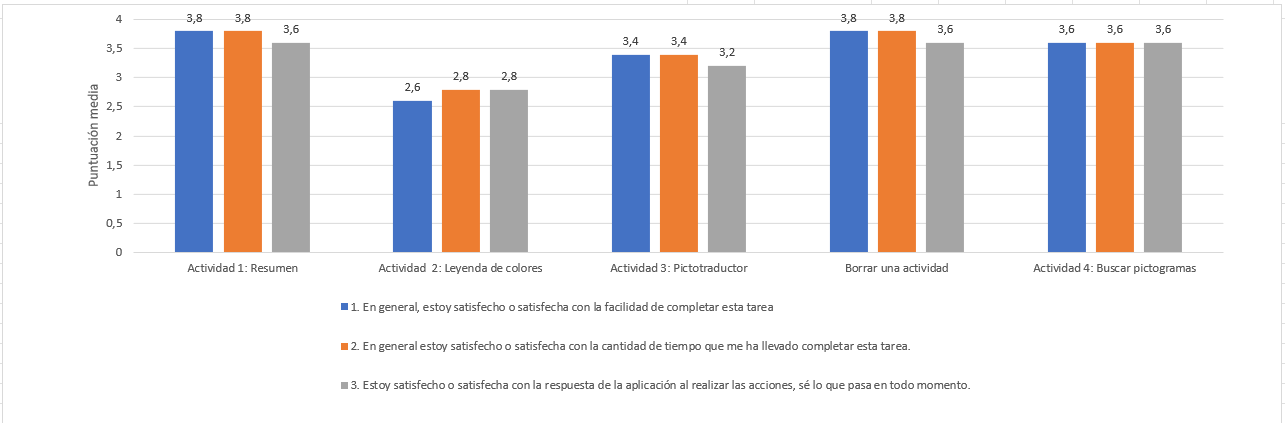
\includegraphics[width=0.8\textwidth]{Evaluacion/GraficaResultadosApuntes.png}
    \caption{Resultados de creación de la hoja de apuntes.}
    \label{fig:resultadosApuntes}
\end{figure}

En cuanto a las preguntas del cuestionario SUS, la puntuación final obtenida fue de 78,5. Esta puntuación indica que el sistema todavía requiere mejoras. Los detalles del cálculo se encuentran en la tabla \ref{tab:puntuacionSUS}.

\begin{table}[H]
    \resizebox{\textwidth}{!}{
        \begin{tabular}{lccc|c|c|}
            \cline{2-6}
            \multicolumn{1}{l|}{}                                                                                                                                                     & \multicolumn{1}{c|}{\textbf{Usuario 1}} & \multicolumn{1}{c|}{\textbf{Usuario 2}} & \textbf{Usuario 3}        & \textbf{Usuario 4}      & \textbf{Usuario 5}      \\ \hline
            \multicolumn{1}{|l|}{\textbf{Creo que usaría esta aplicación frecuentemente.}}                                                                                            & \multicolumn{1}{c|}{5}                  & \multicolumn{1}{c|}{4}                  & 4                         & 5                       & 2                       \\ \hline
            \multicolumn{1}{|l|}{\textbf{Encontré la aplicación innecesariamente compleja}}                                                                                           & \multicolumn{1}{c|}{1}                  & \multicolumn{1}{c|}{2}                  & 2                         & 1                       & 3                       \\ \hline
            \multicolumn{1}{|l|}{\textbf{Creo que la aplicación es fácil de usar}}                                                                                                    & \multicolumn{1}{c|}{4}                  & \multicolumn{1}{c|}{4}                  & 4                         & 5                       & 3                       \\ \hline
            \multicolumn{1}{|l|}{\textbf{\begin{tabular}[c]{@{}l@{}}Creo que necesitaría la ayuda de una persona con \\ conocimientos técnicos para usar la aplicación\end{tabular}}} & \multicolumn{1}{c|}{5}                  & \multicolumn{1}{c|}{1}                  & 1                         & 1                       & 2                       \\ \hline
            \multicolumn{1}{|l|}{\textbf{Las funciones de la aplicación están bien integradas}}                                                                                       & \multicolumn{1}{c|}{5}                  & \multicolumn{1}{c|}{4}                  & 4                         & 5                       & 2                       \\ \hline
            \multicolumn{1}{|l|}{\textbf{Creo que la aplicación es muy confusa}}                                                                                                      & \multicolumn{1}{c|}{2}                  & \multicolumn{1}{c|}{2}                  & 2                         & 1                       & 3                       \\ \hline
            \multicolumn{1}{|l|}{\textbf{\begin{tabular}[c]{@{}l@{}}Creo que la mayoría de la gente aprendería a \\ usar la aplicación muy rápidamente\end{tabular}}}                 & \multicolumn{1}{c|}{5}                  & \multicolumn{1}{c|}{4}                  & 5                         & 4                       & 4                       \\ \hline
            \multicolumn{1}{|l|}{\textbf{Encuentro la aplicación muy complicada de utilizar}}                                                                                         & \multicolumn{1}{c|}{1}                  & \multicolumn{1}{c|}{5}                  & 1                         & 1                       & 2                       \\ \hline
            \multicolumn{1}{|l|}{\textbf{Me siento confiado o confiada al utilizar la aplicación}}                                                                                    & \multicolumn{1}{c|}{5}                  & \multicolumn{1}{c|}{5}                  & 5                         & 5                       & 3                       \\ \hline
            \multicolumn{1}{|l|}{\textbf{\begin{tabular}[c]{@{}l@{}}Necesito aprender muchas cosas antes de poder \\ utilizar la aplicación\end{tabular}}}                            & \multicolumn{1}{c|}{1}                  & \multicolumn{1}{c|}{1}                  & 1                         & 4                       & 2                       \\ \hline
            \multicolumn{1}{|c|}{\textbf{Resultado}}                                                                                                                                  & \multicolumn{1}{c|}{85}                 & \multicolumn{1}{c|}{75}                 & \multicolumn{1}{c|}{87,5} & \multicolumn{1}{c|}{90} & \multicolumn{1}{c|}{55} \\ \hline
                                                                                                                                                                                      & \multicolumn{1}{l}{}                    & \multicolumn{1}{l}{}                    & \multicolumn{1}{l|}{}     & \textbf{Media:}         & \textbf{78,5}           \\ \cline{5-6}
        \end{tabular}
    }
    \caption{Resultado del cuestionario SUS}
    \label{tab:puntuacionSUS}
\end{table}

En cuanto a las preguntas de debriefing, las distintas respuestas se muestran en la Tabla \ref{tab:resultadosDebriefing}.

\begin{table}[H]
    \resizebox{\textwidth}{!}{
    \begin{tabular}{c|l|l|l|l|l|l|}
    \cline{2-7}
    \multicolumn{1}{l|}{}                    & \multicolumn{1}{c|}{\textbf{¿Qué te ha parecido la aplicación?}}                                                                                                                                                                                                                                                            & \multicolumn{1}{c|}{\textbf{¿Qué es lo que más te ha gustado?}}                                                                                                                                                                                                                                                                                    & \multicolumn{1}{c|}{\textbf{¿Qué es lo que menos te ha gustado?}}                                                                                                                                                                                                                                                                                            & \multicolumn{1}{c|}{\textbf{¿Echas de menos alguna funcionalidad?}}                                                                                                                                                & \multicolumn{1}{c|}{\textbf{¿Te sobra alguna funcionalidad?}}                                                                                                                                          & \multicolumn{1}{c|}{\textbf{¿Algo más que quieras añadir?}}                                                                                                \\ \hline
    \multicolumn{1}{|l|}{\textbf{Usuario 1}} & \begin{tabular}[c]{@{}l@{}}Me parece que está muy bien \\ y que es muy útil\end{tabular}                                                                                                                                                                                                                                    & \begin{tabular}[c]{@{}l@{}}Las opciones que te presentan, \\ algunas de ellas muy útiles y\\ necesarias como la posibilidad de \\ hacer los resúmenes, el buscar\\ pictogramas en un texto, etc. \\ Son muy novedosas y la verdad \\ que son muy intuitivas \\ todas las opciones\end{tabular}                                                     & \begin{tabular}[c]{@{}l@{}}El no poder editar el texto como \\ si fuese un word, cada ejercicio \\ se ponía en una caja y en la primera \\ actividad se me han movido todos, \\ intentando quitar la numeración se ha \\ borrado un ejercicio y he echado en \\ falta una opción de deshacer o \\ ir hacia atrás.\end{tabular}                               & \begin{tabular}[c]{@{}l@{}}he echado en falta una opción \\ de deshacer o ir hacia atrás.\end{tabular}                                                                                                             & No en principio no                                                                                                                                                                                     & \begin{tabular}[c]{@{}l@{}}Esta genial, sin duda a \\ mi me gustaría usarla\end{tabular}                                                                   \\ \hline
    \multicolumn{1}{|c|}{\textbf{Usuario 2}} & \begin{tabular}[c]{@{}l@{}}Me ha parecido una herramienta \\ muy útil para el profesorado. \\ No solo para atender \\ a alumnos con necesidades, \\ sino para emplearlo en el día \\ a día. Es muy sencilla e intuitiva \\ y nos podría ahorran gran cantidad \\ de tiempo en la preparación \\ de materiales.\end{tabular} & \begin{tabular}[c]{@{}l@{}}Las opciones de \\ ejercicios, especialmente la \\ sopa de letras, completar huecos\\ en blanco y relacionar conceptos. \\ Estos últimos años he empleado \\ mucho tiempo en la creación de \\ exámenes de este tipo. Si hubiera \\ tenido esta aplicación el tiempo \\ invertido habría sido mucho menor.\end{tabular} & \begin{tabular}[c]{@{}l@{}}La leyenda de colores. \\ Pensé que habría \\ una opción de meter \\ instantáneamente \\ cada categoría en un \\ color y he tenido que \\ ir uno por uno desde \\ el formato \\ del texto. Puede que \\ exista una opción, \\ pero yo no la encontré.\end{tabular}                                                                & \begin{tabular}[c]{@{}l@{}}Sí. Una herramienta de deshacer. \\ He borrado por error un \\ ejercicio y no he encontrado la manera \\ de volver atrás. He tenido \\ que realizar el ejercicio de nuevo.\end{tabular} &                                                                                                                                                                                                        &                                                                                                                                                            \\ \hline
    \multicolumn{1}{|c|}{\textbf{Usuario 3}} & \begin{tabular}[c]{@{}l@{}}Bastante completa, aunque \\ echo en falta un icono \\ de "ayuda" que explique \\ brevemente cómo funciona\\ cada ejercicio, algo así \\ como: pasos a seguir; \\ esquemático, simple...\end{tabular}                                                                                            & \begin{tabular}[c]{@{}l@{}}Una vez que he \\ entendido cómo \\ funciona el ejercicio, \\ la facilidad \\ con que se \\ redacta/ realiza.\end{tabular}                                                                                                                                                                                              & \begin{tabular}[c]{@{}l@{}}Supongo   que no es \\ algo "achacable" a la aplicación, \\ sino al cuestionario en sí, y al hecho \\ de haber "pinchado" en el enlace de la \\ aplicación, haber redactado mi \\ propio examen y, después, al \\ pasar de página, ver que se \\ proponían unos ejercicios \\ tipo. He perdido mucho tiempo en esto.\end{tabular} & \begin{tabular}[c]{@{}l@{}}Lo que he comentado. Algún icono \\ de "ayuda" que explique \\ brevemente la forma en que se \\ realiza el ejercicio.\end{tabular}                                                      & \begin{tabular}[c]{@{}l@{}}Creo que el "traductor a \\ pictogramas" no es necesario.\\ Se suelen insertar pictogramas \\ en un texto, pero no traducir una \\ por una todas las palabras.\end{tabular} & \begin{tabular}[c]{@{}l@{}}Espero que este año se \\ puedan utilizar los enlaces \\ proporcionados para su uso y \\ la página esté operativa.\end{tabular} \\ \hline
    \multicolumn{1}{|c|}{\textbf{Usuario 4}} & \begin{tabular}[c]{@{}l@{}}Me parece muy útil para la \\ elaboración de actividades.\end{tabular}                                                                                                                                                                                                                           & \begin{tabular}[c]{@{}l@{}}La variedad de \\ opciones \\ que permite realizar.\end{tabular}                                                                                                                                                                                                                                                        & \begin{tabular}[c]{@{}l@{}}La parte de Matemáticas la considero \\ algo confusa.\end{tabular}                                                                                                                                                                                                                                                                & Me parecen suficientes.                                                                                                                                                                                            & No.                                                                                                                                                                                                    & \multicolumn{1}{c|}{}                                                                                                                                      \\ \hline
    \multicolumn{1}{|c|}{\textbf{Usuario 5}} & \begin{tabular}[c]{@{}l@{}}Me parece interesante, \\ pero está muy limitada \\ y a mi la parte de traducir a \\ pictogramas no me ha \\ funcionado. Tampoco he \\ podido ver como resume \\ un texto porque no me \\ lo ha hecho. La idea está \\ muy bien pero falta que \\ funcione correctamente.\end{tabular}           & \begin{tabular}[c]{@{}l@{}}Poder hacer crucigramas \\ con tanta facilidad aunque ya \\ existen aplicaciones \\ donde lo hacemos.\end{tabular}                                                                                                                                                                                                      & \begin{tabular}[c]{@{}l@{}}El ejercicio de formulación \\ matemática.\end{tabular}                                                                                                                                                                                                                                                                           & \begin{tabular}[c]{@{}l@{}}Los pictogramas. No he podido \\ visualizar nada.\end{tabular}                                                                                                                          & No                                                                                                                                                                                                     & \begin{tabular}[c]{@{}l@{}}Que se puedan mover los ejercicios. \\ El documento que no sea tan cerrado\end{tabular}                                         \\ \hline
    \end{tabular}
    }
    \caption{Resultados de las preguntas de debriefing}
    \label{tab:resultadosDebriefing}
\end{table}

\section{Conclusiones}\label{sec:conclusionesEvaluacion}
Tras evaluar la aplicación web AdaptaMaterialEscolar 2.0, hemos determinado que, aunque existen áreas de mejora, el sistema presenta una usabilidad satisfactoria, con una puntuación de 78.5 sobre 100 (Tabla \ref{tab:puntuacionSUS}).

En cuanto a las funcionalidades para generar ejercicios, la evaluación refleja que la facilidad para completar las tareas es alta, ya que todas las puntuaciones promedio para la pregunta ``facilidad de completar esta tarea'' están por encima de 4 (Figura \ref{fig:resultadosExamen}). La cantidad de tiempo requerido para completar las tareas también es en su mayoría satisfactoria, ya que todas las puntuaciones promedio para la pregunta ``cantidad de tiempo que me ha llevado completar esta tarea'' son iguales o superiores a 4 (Figura \ref{fig:resultadosExamen}). Las puntuaciones promedio para la pregunta ``respuesta de la aplicación al realizar las acciones, sé lo que pasa en todo momento'' son de 5, lo cual indica que los usuarios están muy satisfechos con la respuesta de la aplicación y su capacidad de comprender lo que ocurre (Figura \ref{fig:resultadosExamen}). Además, observamos que el ejercicio de desarrollo, la modificación del ejercicio de desarrollo, el ejercicio de completar huecos, el ejercicio de sopa de letras y el ejercicio para espacio para dibujar obtienen la puntuación más alta, mientras que el ejercicio de completar huecos cuenta con la puntuación más baja.

Por otro lado, las funcionalidades para crear apuntes también reflejan una alta facilidad para completar las tareas, ya que todas las actividades tienen una puntuación promedio superior a 3 (en una escala del 1 al 5) (Figura \ref{fig:resultadosApuntes}). Esto indica que los usuarios se sienten satisfechos con la facilidad de completar las tareas en general. Además, la cantidad de tiempo requerido para completar las tareas también es en su mayoría satisfactoria, ya que las puntuaciones promedio son superiores a 3 para todas las actividades (Figura \ref{fig:resultadosApuntes}). En cuanto a la respuesta de la aplicación al realizar acciones y la comprensión de lo que sucede en todo momento, las puntuaciones son consistentes, con valores que rondan entre 3.2 y 3.8 (Figura \ref{fig:resultadosApuntes}). Esto indica que los usuarios tienen una percepción generalmente satisfactoria de la respuesta de la aplicación y su comprensión de las acciones realizadas. Cabe destacar que la funcionalidad para generar resumen y borrar una actividad obtienen la puntuación más alta, mientras que la leyenda de colores cuenta con la puntuación más baja (Figura \ref{fig:resultadosApuntes}).

Por último, es importante destacar que los usuarios se mostraron más cómodos con las funcionalidades relacionadas con la generación de ejercicios de examen (Figura \ref{fig:graficaComparativaEjerciciosApuntes}) que con las de adaptación de texto.

\begin{figure}[H]
    \centering
    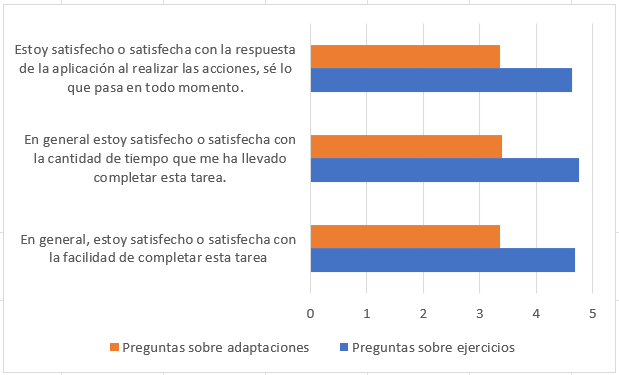
\includegraphics[width=0.75\textwidth]{Evaluacion/GraficaComparativaEjerciciosApuntes.png}
    \caption{Gráfica comparativa entre ejercicios y apuntes.}
    \label{fig:graficaComparativaEjerciciosApuntes}
\end{figure}